\documentclass{article}

\input{lstlistingdef}

% ------------------------------
% PACKAGES
% ------------------------------
\usepackage{fancyhdr}
\usepackage{extramarks}
\usepackage{amsmath, amsthm, amsfonts}
\usepackage{tikz}
\usepackage[plain]{algorithm}
\usepackage{algpseudocode}
\usepackage{hyperref}
\usepackage{xcolor}
\usepackage{graphicx}
\usepackage{enumitem}

% ------------------------------
% HYPERREF CONFIG
% ------------------------------
\hypersetup{
	colorlinks = true,
	linkcolor  = red!60!black,
	citecolor  = blue!50!black,
	urlcolor   = blue!80!black
}

\usetikzlibrary{automata,positioning}

% ------------------------------
% PAGE SETUP
% ------------------------------
\topmargin=-0.45in
\evensidemargin=0in
\oddsidemargin=0in
\textwidth=6.5in
\textheight=9.0in
\headsep=0.25in
\linespread{1.1}

\pagestyle{fancy}
\rhead{\hmwkClass: \hmwkTitle}
\lfoot{\lastxmark}
\cfoot{\thepage}
\renewcommand\headrulewidth{0.4pt}
\renewcommand\footrulewidth{0.4pt}

\setlength\parindent{0pt}

% ------------------------------
% SECTION NUMBERING
% ------------------------------
\setcounter{secnumdepth}{2}  % <--- Abilita numerazione delle sezioni

% ------------------------------
% CUSTOM ENUMERATE STYLE
% ------------------------------
\setlist[enumerate,1]{label=\textbf{(\alph*)}, leftmargin=2em} % lettere (a), (b), ...
\setlist[enumerate,2]{label=\textbf{(\roman*)}, leftmargin=3em} % sotto-elenchi (i), (ii), ...

% ------------------------------
% HOMEWORK DETAILS
% ------------------------------
\newcommand{\hmwkTitle}{Homework 1}
\newcommand{\hmwkSubtitle}{Bring up your robot}
\newcommand{\hmwkClass}{Robotics Lab}
\newcommand{\hmwkClassInstructor}{Mario Selvaggio}
\newcommand{\hmwkAuthorName}{
	Student1: \url{https://github.com/carlobarone00} \\ 
	Student2: \url{https://github.com/Moreno-Zaccara} \\ 
	Student3: \url{https://github.com/Student3} \\ 
	Student4: \url{https://github.com/Student4}
}

% ------------------------------
% TITLE
% ------------------------------
\title{
	\vspace{2in}
	\textmd{\textbf{\hmwkClass:\ \hmwkTitle}}\\
	\normalsize\vspace{0.1in}\small{\hmwkSubtitle}\\
	\vspace{3in}
}
\author{\hmwkAuthorName}
\date{}
\usepackage{subcaption}
\usepackage{float}
% ------------------------------
% DOCUMENT
% ------------------------------
\begin{document}

\maketitle
\pagebreak

\section{Robot Visualization Setup in RViz}
\begin{enumerate}
	\item creating a launch folder within the \lstinline{armando_description} package containing the launch file named \lstinline{armando_display.launch}
    \begin{figure}[h]
    \centering
    \begin{subfigure}[t]{0.48\linewidth}
        \centering
        \includegraphics[width=\linewidth]{img/1.1.png}
        \caption{Launch folder created inside \texttt{armando\_description}}
        \label{fig:1.1}
    \end{subfigure}
    \hfill
    \begin{subfigure}[t]{0.48\linewidth}
        \centering
        \includegraphics[width=\linewidth]{img/armand_desc_launch_py.png}
        \caption{Content of the \texttt{armando\_display.launch} file}
        \label{fig:armand_desc_launch_py}
    \end{subfigure}
    \caption{Creation of the launch folder and corresponding launch file in \texttt{armando\_description}}
    \label{fig:launch_setup}
    \end{figure}
    
\noindent Specifically, the launch file has the structure shown in the following image:

\begin{figure}[h]
    \centering
    \includegraphics[width=0.8\linewidth]{img/armando_desc_launch.png}
    \caption{Structure of the \texttt{armando\_display.launch} file.}
    \label{fig:armando_desc_launch}
\end{figure}

\clearpage
\noindent As shown in the following figure, the launch file initializes three essential ROS~2 nodes: \\
the \lstinline{robot_state_publisher}, the \lstinline{joint_state_publisher}, and the \lstinline{rviz2} node. \\ 
The \lstinline{robot_state_publisher} node is responsible for broadcasting the transformations between the robot’s links 
based on the URDF description. The \lstinline{joint_state_publisher} node publishes the current joint positions, 
either manually specified or read from hardware interfaces, while \lstinline{rviz2} provides the visualization environment.

\vspace{0.5em}
\noindent To correctly visualize the robot model in RViz, we configured the display by setting the \textbf{Fixed Frame} parameter 
to the robot’s reference frame and by adding a \lstinline{Robot Model} display to render the URDF description. 
This ensures that all subsequent transformations and sensor data are aligned with the correct reference frame.

\begin{figure}[h]
    \centering
    \includegraphics[width=0.6\linewidth]{img/rviz_robot.png}
    \caption{Visualization of the Armando robot model in RViz after configuring the \texttt{Robot Model} display.}
    \label{fig:rviz_robot}
\end{figure}

\item \textbf{RViz Configuration File}

\noindent Inside the \lstinline{config} directory of the \lstinline{armando_description} package, 
we added a configuration file named \lstinline{config.rviz}. This file stores the customized RViz layout, 
including the loaded displays, visual parameters, and the selected fixed frame. 

\begin{figure}[h]
    \centering
    \includegraphics[width=0.3\linewidth]{img/nodo_rviz.png}
    \caption{RViz node configuration for automatic robot model visualization.}
    \label{fig:nodo_rviz}
\end{figure}

\item \textbf{Simplification of Collision Models}

\noindent To improve simulation performance and stability, we replaced the detailed collision meshes in the URDF 
with simplified \textit{primitive geometries}. In particular, we used box-shaped elements as approximations of 
the original link volumes. This approach maintains reasonable physical accuracy while significantly reducing 
computational cost during collision detection.

\vspace{0.5em}
\noindent The collision properties for each link are defined by the \lstinline{box size} attribute in the URDF file. 
An example of one link’s collision box definition is shown below, but the same procedure was iteratively applied 
to every joint and link of the robot model.

\begin{figure}[H]
    \centering
    \includegraphics[width=0.8\linewidth]{img/Collision_mesh.png}
    \caption{Example of a collision box definition within the URDF file.}
    \label{fig:Collision_mesh}
\end{figure}

\noindent The resulting model, shown in the following figure, demonstrates the simplified collision geometry of the robot. 
This representation enables efficient collision checking while preserving the robot’s kinematic structure for 
both visualization and physical simulation purposes.

\begin{figure}[h]
    \centering
    \includegraphics[width=0.3\linewidth]{img/armando_collision.png}
    \caption{Final simplified collision model of the Armando robot.}
    \label{fig:armando_collision}
\end{figure}

\end{enumerate}
\pagebreak
\section{Setting Up the Gazebo Simulation and Hardware Interface}
\begin{enumerate}
    \item Creating a package using the terminal by using the following command line:
    \begin{center}
        \texttt{ros2 pkg create --build-type \lstinline{ament_cmake armando_gazebo}}
    \end{center}

\noindent Once created, since the \lstinline{ros2 pkg create} command do not create all the folders we need, we also made sure to add the launch directory (inside the package that we jsut created) with the following command line:

  \begin{center}
        \texttt{mkdir launch}
    \end{center}

\noindent Once done the previous steps, our package will have the following stuff inside:
    \begin{figure}[H]
    \centering
    \includegraphics[width=0.9\linewidth]{img/armando_gazebo.png}
    \caption{Structure of the \texttt{armando\_gazebo} package with the launch folder added.}
    \label{fig:armando_gazebo}
    \end{figure}
    
\noindent The \lstinline{armando_world.launch.py} file is included inside the launch directory and it's filled with commands to load the URDF file into the \lstinline{/robot_description} topic and spawn the robot using the \lstinline{create node} in the \lstinline{ros_gz_sim} package:

    \begin{figure}[H]
    \centering
    \includegraphics[width=0.9\linewidth]{img/armando_gazebo_launch.png}
    \caption{Launch file for loading the robot model and spawning it in Gazebo.}
    \label{fig:armando_gazebo_launch}
    \end{figure}
    
\noindent The robot gets spawned thanks to the following code line:

    \begin{figure}[H]
        \centering
        \includegraphics[width=0.8\linewidth]{img/gazebo_launch1.png}
        \label{fig:gazebo_launch1}
        \caption{Spawning of the Robot code - 1}
        \label{fig:spawning_robot_code_1}
    \end{figure}
        \begin{figure}[H]
        \centering
        \includegraphics[width=0.8\linewidth]{img/gazebo_launch2.png}
        \caption{Spawning of the Robot code - 2}
        \label{fig:spawning_robot_code_2}
    \end{figure}
        \begin{figure}[H]
        \centering
        \includegraphics[width=0.8\linewidth]{img/gazebo_launch3.png}
        \caption{Spawning of the Robot code - 3}
        \label{fig:spawning_robot_code_3}
    \end{figure}

\clearpage
\item To enable position control of the robot’s joints in simulation, we added a 
\lstinline{PositionJointInterface} named \lstinline{HardwareInterface_Ignition}, 
implemented using the \lstinline{ros2_control} framework. This interface allows the controllers to 
send and receive commands corresponding to the robot’s joint positions, bridging the gap between 
the simulated hardware (in Gazebo) and the ROS~2 control nodes.

\begin{figure}[H]
    \centering
    \includegraphics[width=0.8\linewidth]{img/PositionJointInterface.png}
    \caption{Definition of the \texttt{PositionJointInterface} within the \texttt{ros2\_control} framework.}
    \label{fig:PositionJointInterface}
\end{figure}

\noindent The hardware interface is defined inside a dedicated file named 
\lstinline{armando_hardware_interface.xacro}, located in the 
\lstinline{armando_description/urdf} directory. This file contains a 
\lstinline{xacro:macro} definition that describes how the robot’s joints are mapped to the 
ROS~2 control interfaces, specifying which joints are actuated and how they interact with the 
simulation backend.

\begin{figure}[H]
    \centering
    \includegraphics[width=0.4\linewidth]{img/armando_hardware_xacro.png}
    \caption{Excerpt from the \texttt{armando\_hardware\_interface.xacro} file showing the macro definition.}
    \label{fig:armando_hardware_xacro}
\end{figure}

\noindent The hardware interface macro is then included within the main 
\lstinline{armando.urdf.xacro} file (previously renamed from \lstinline{armando.urdf}) 
using the \lstinline{xacro:include} directive. This inclusion makes the hardware interface 
part of the robot’s unified URDF structure, allowing the controller manager to load and initialize 
the correct control resources during simulation startup.

\begin{figure}[H]
    \centering
    \includegraphics[width=0.9\linewidth]{img/hardware_include.png}
    \caption{Inclusion of the hardware interface macro inside the main URDF description.}
    \label{fig:hardware_include}
\end{figure}


\item In the main \lstinline{armando.urdf.xacro} file, the Gazebo ROS~2 Control plugin is included to load and manage the joint position controllers.

\begin{figure}[H]
    \centering
    \includegraphics[width=0.5\linewidth]{img/yaml_include.png}
    \caption{Inclusion of the controller configuration YAML file in the URDF.}
    \label{fig:yaml_include}
\end{figure}

\noindent The YAML file defines the parameters and interfaces for both the \lstinline{joint_state_broadcaster} and the \lstinline{position_controller}.

\begin{figure}[H]
    \centering
    \includegraphics[width=0.5\linewidth]{img/yaml.png}
    \caption{YAML configuration defining the robot controllers.}
    \label{fig:yaml}
\end{figure}

\noindent The controllers are spawned in the \lstinline{armando_world.launch.py} file inside the \lstinline{armando_gazebo/launch} directory.

\begin{figure}[H]
    \centering
    \includegraphics[width=0.7\linewidth]{img/broadcaster_position.png}
    \caption{Commands for spawning the joint state broadcaster and position controllers.}
    \label{fig:broadcaster_position}
\end{figure}

\noindent The Gazebo simulation is launched with:
\begin{center}
\small
\texttt{ros2 launch armando\_gazebo armando\_world.launch.py}
\end{center}

\noindent When started, the terminal confirms that the hardware interface and controllers are correctly loaded.

\begin{figure}[H]
    \centering
    \includegraphics[width=0.5\linewidth]{img/position_controller.png}
    \caption{Verification of the controllers successfully loaded in simulation.}
    \label{fig:position_controller}
\end{figure}
\end{enumerate}
\pagebreak

\section{Camera Setup and Visualization in Gazebo}
\begin{enumerate}
\item Adding a \lstinline{carmera_link} and a \lstinline{camera_joint} of fixed type in order to define the link and the join used to setup the camera for the Gazebo environment:

        \begin{figure}[H]
        \centering
        \includegraphics[width=0.5\linewidth]{img/camera_joint_link.png}
        \label{fig:camera_joint_link}
        \caption{Camera Code}
    \end{figure}

\noindent The \lstinline{camera_link} and the \lstinline{camera_joint} are both included inside the \lstinline{armando.urdf.xacro} file. The values for size and position have been chosen in orded to let the camera be visible in the simulation environment, while the rpy axis have been chosen in order to let our camera be oriented from the bottom to the top.

        \begin{figure}[H]
        \centering
        \includegraphics[width=0.35\linewidth]{img/robot_camera.png}
        \label{fig:robot_camera}
        \caption{Camera in the Robot}
        \end{figure}

\item The \lstinline{armando_camera.xacro} file was created inside the \lstinline{armando_gazebo/urdf} folder.

\begin{figure}[H]
    \centering
    \includegraphics[width=0.5\linewidth]{img/camera_xacro_folder.png}
    \caption{Location of the \texttt{armando\_camera.xacro} file in the package structure.}
    \label{fig:camera_xacro_folder}
\end{figure}

\noindent This file defines the camera sensor using a \lstinline{xacro:macro} and includes the necessary Gazebo plugins for image publishing.

\begin{figure}[H]
    \centering
    \includegraphics[width=0.5\linewidth]{img/camera_macro.png}
    \caption{Macro definition and plugin configuration inside \texttt{armando\_camera.xacro}.}
    \label{fig:camera_macro}
\end{figure}

\noindent The macro is included in the main \lstinline{armando.urdf.xacro} file using the \lstinline{xacro:include} directive.

\begin{figure}[H]
    \centering
    \includegraphics[width=0.5\linewidth]{img/macro_include.png}
    \caption{Inclusion of the camera macro in the main URDF description.}
    \label{fig:macro_include}
\end{figure}

\item By using the command line \lstinline{ros2 run rqt_image_view rqt_image_view} it's possible to see that the topic is correctly published, in fact the camera also shows what it's pointing to:
    \begin{figure}[htpb]
        \centering
        \includegraphics[width=0.5\linewidth]{img/camera_image.png}
        \label{fig:camera_image}
        \caption{Point of view of the Camera}
    \end{figure}

\noindent The brige used to link the camera is given by the following code: 
    \begin{figure}[htpb]
        \centering
        \includegraphics[width=0.5\linewidth]{img/camera_bridge.png}
        \label{fig:camera_bridge}
        \caption{Bridge to link the camera}
\end{figure}
\end{enumerate}
\pagebreak

\section{Design and Implementation of the ROS 2 Control Node}
\begin{enumerate}
    \item Creating the \lstinline{armando_controller} package with the specifications given by the homework using the proper command on the terminal:
       \begin{center}
       \small
        \texttt{ros2 pkg create --build-type ament-cmake --node-name
        \lstinline{arm_controler_node} --dependencies rclcpp \lstinline{sensor_msgs std_msgs}}
        \end{center}
\noindent Once done, we modified the \lstinline{CMakeLists.txt} and the \lstinline{package.xml} files in order to compile the node: 
    \begin{figure}[h]
        \centering
        \includegraphics[width=0.5\linewidth]{img/controller_cmake.png}
        \label{fig:controller_cmake}
    \end{figure}
        \begin{figure}[h]
        \centering
        \includegraphics[width=0.5\linewidth]{img/controller_package.png}
        \label{fig:controller_package}
    \end{figure}
    \item We created a subscriber to the topic \texttt{joint\_states} using the message type \texttt{sensor\_msgs/msg/JointState}. 
    This subscriber is responsible for receiving the current joint positions of the robot and printing them in the terminal each time a new message is published on the topic. 

    The subscriber was defined as follows:

\begin{lstlisting}[language=C++]
    joint_state_sub_ = this->create_subscription<sensor_msgs::msg::JointState>(
    "joint_states",
    10,
    std::bind(&ArmControllerNode::jointStateCallback, this, _1));
\end{lstlisting}
    
The associated callback function, \texttt{jointStateCallback()}, iterates through all joint positions and prints their values:
\begin{lstlisting}[language=C++]
    for (size_t i = 0; i < msg->position.size(); ++i) {
    RCLCPP_INFO(this->get_logger(), "  joint[%zu]: %.3f", i, msg->position[i]);
    }
\end{lstlisting}

In this way, every time a new joint state message is received, the current position of each joint is displayed in the console, 
allowing real-time monitoring of the robot’s motion state.
\item We defined a publisher named \texttt{position\_comm\_pub} that publishes sequential joint position commands 
to the topic \texttt{/position\_controller/commands}. This topic uses the message type \texttt{std\_msgs/msg/Float64MultiArray}, 
which allows sending an array of target joint positions to the robot’s position controller.

The publisher was created as follows:

\begin{lstlisting}[language=C++]
position_comm_pub_ = this->create_publisher<std_msgs::msg::Float64MultiArray>(
    "/position_controller/commands",
    10);
\end{lstlisting}

The predefined sequence of commands was defined in a vector structure:

\begin{lstlisting}[language=C++]
command_sequence_ = {
    {0.0, 0.0, 0.2, 0.0},
    {0.0, 0.3, 0.2, 0.0},
    {0.0, 0.0, 0.0, 0.0},
    {0.0, 0.0, -0.2, 0.0}
};
\end{lstlisting}

Each command is published through the function \texttt{publishCommand()}, which sends the next element of the sequence to the controller:

\begin{lstlisting}[language=C++]
std_msgs::msg::Float64MultiArray msg;
msg.data = command_sequence_[command_index_];   
position_comm_pub_->publish(msg);
\end{lstlisting}
\item 
At first, let's modify \texttt{armando\_controller.cpp} in order to allow 
the  node to publish on the right topic and 
with the corresponding type of data according to the user's controller choice.

\begin{figure}[H] % ✅ aggiunto [h!] per forzare il posizionamento
  \centering
  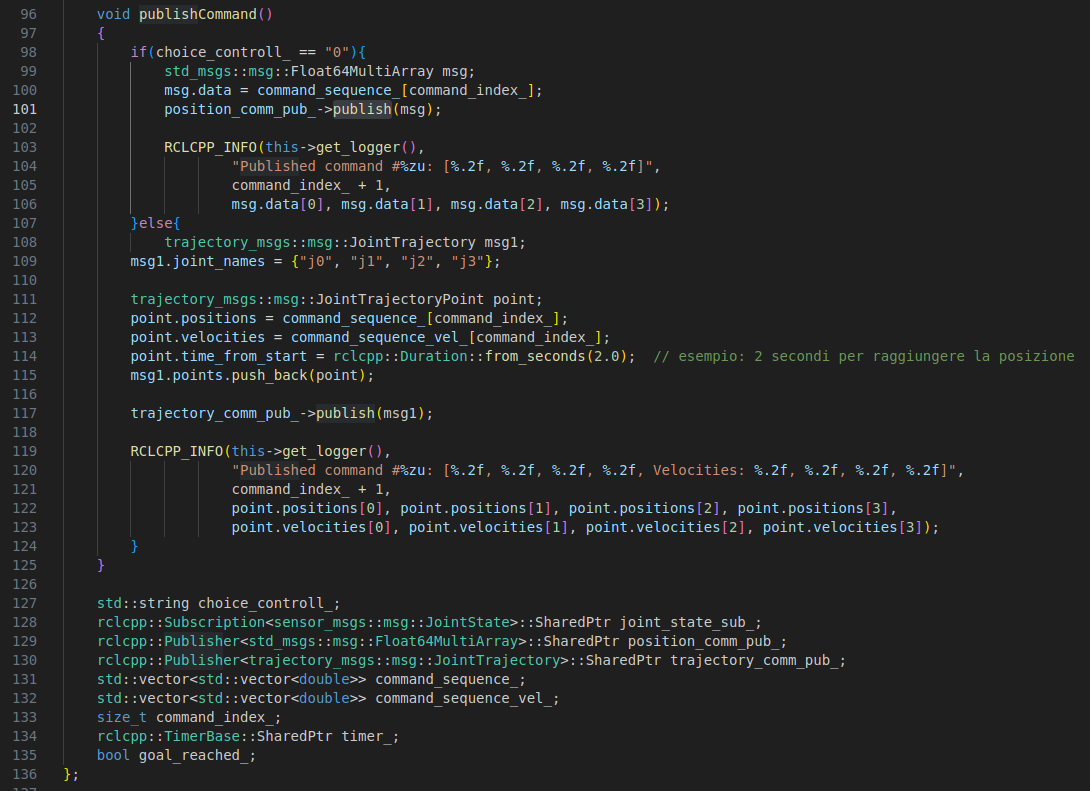
\includegraphics[width=1\textwidth]{Images/4D_1.png} % nome file e larghezza
  \caption{Structure of the publishCommand after modification.} % ✅ didascalia
  \label{fig:publishCommand}
\end{figure}
\begin{figure}[H] % ✅ aggiunto [h!] per forzare il posizionamento
  \centering
  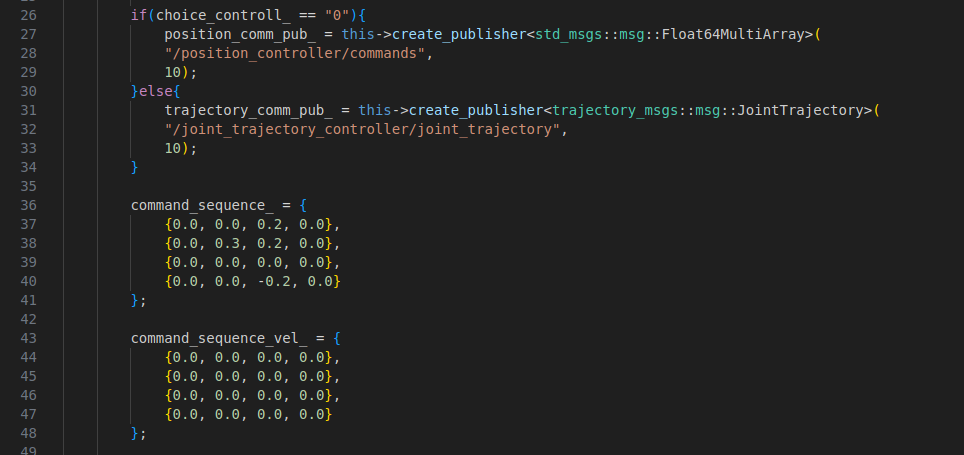
\includegraphics[width=1\textwidth]{Images/4D_2_1.png} % nome file e larghezza
  \caption{ArmControllerNode constructor editings} % ✅ didascalia
  \label{fig:publishCommand}
\end{figure}

In order to use the \texttt{joint\_trajectory\_controller}, it must be loaded and configured 
in \texttt{armando\_world.launch.py}, and its configuration must be added in 
\texttt{armando\_controllers.yaml}.

\begin{figure}[H] % ✅ aggiunto [h!] per forzare il posizionamento
  \centering
  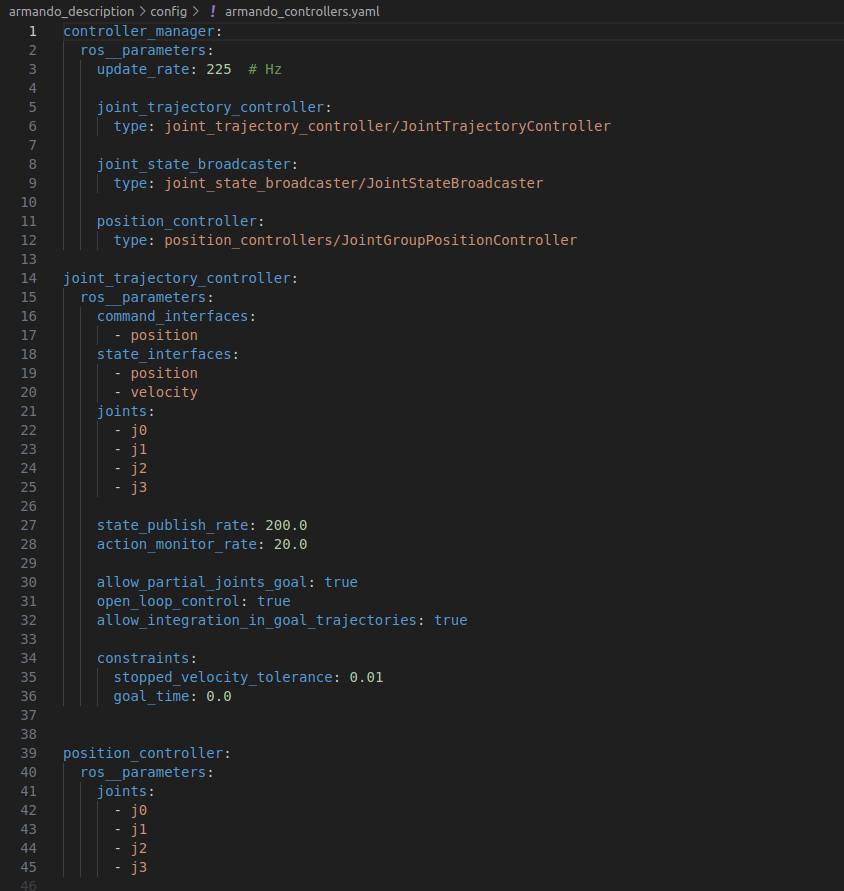
\includegraphics[width=1\textwidth]{Images/4D_2.png} % nome file e larghezza
  \caption{\texttt{armando\_controllers.yaml} after \texttt{joint\_trajectory\_controller} configuration adding } % ✅ didascalia
  \label{fig:publishCommand}
\end{figure}
\begin{figure}[H] % ✅ aggiunto [h!] per forzare il posizionamento
  \centering
  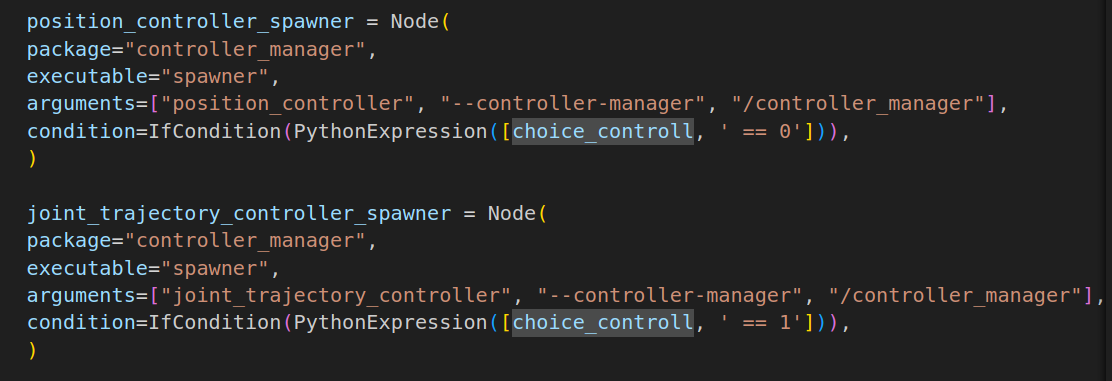
\includegraphics[width=1\textwidth]{Images/4D_3.png} % nome file e larghezza
  \caption{editings in the controllers loadings to add \texttt{joint\_trajectory\_controller} and make they dependet on \texttt{choice\_control} parameter in  \texttt{armando\_world.launch.py}  .} % ✅ didascalia
  \label{fig:publishCommand}
In the 

  
\end{figure}

As with the other two controllers, the \texttt{joint\_trajectory\_controller} 
also waits for the robot to spawn in Gazebo in the same fashion. 
Below is the definition of the argument \texttt{choice\_control\_arg}, 
which allows the user to choose the controller from the command line.

\begin{figure}[H] % ✅ aggiunto [h!] per forzare il posizionamento
  \centering
  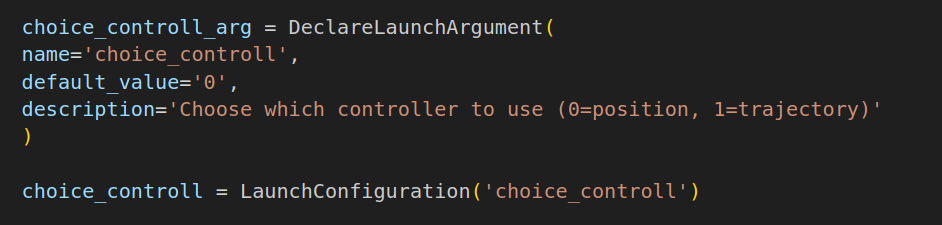
\includegraphics[width=1\textwidth]{Images/4D_4.png} % nome file e larghezza
  \caption{Definition of the argument \texttt{choice\_control\_arg} in 
\texttt{armando\_world.launch.py.}} % ✅ didascalia
  \label{fig:publishCommand}
\end{figure}

Always in \texttt{armando\_world.launch.py}, the \texttt{armando\_controller.cpp} 
is launched by the same delay function as the other controllers, 
of course after them, passing to it the \texttt{choice\_control} argument.
\begin{figure}[H] % ✅ aggiunto [h!] per forzare il posizionamento
  \centering
  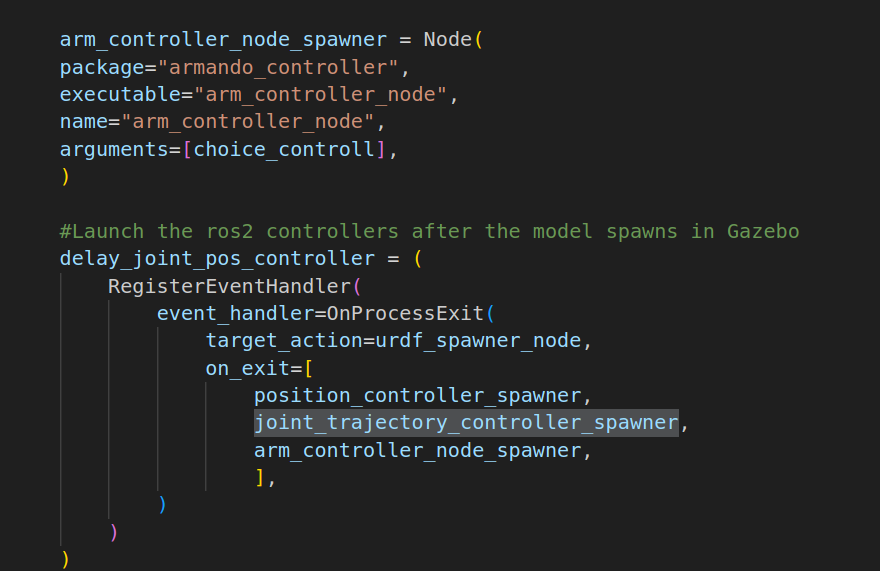
\includegraphics[width=1\textwidth]{Images/4D_5.png} % nome file e larghezza
  \caption{\texttt{armando\_controller.cpp} launch } % ✅ didascalia
  \label{fig:publishCommand}
\end{figure}
If the user selects \texttt{choice\_control} as 0, the 
\texttt{position\_controller\_spawner} will be launched; 
if it is 1, the \texttt{joint\_trajectory\_controller\_spawner} will be launched.

\begin{figure}[H] % ✅ aggiunto [h!] per forzare il posizionamento
  \centering
  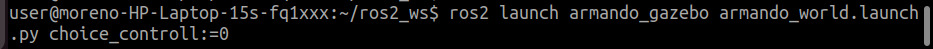
\includegraphics[width=1\textwidth]{Images/4D_6.jpeg} % nome file e larghezza

  \label{fig:publishCommand}
\end{figure}
\begin{figure}[H] % ✅ aggiunto [h!] per forzare il posizionamento
  \centering
  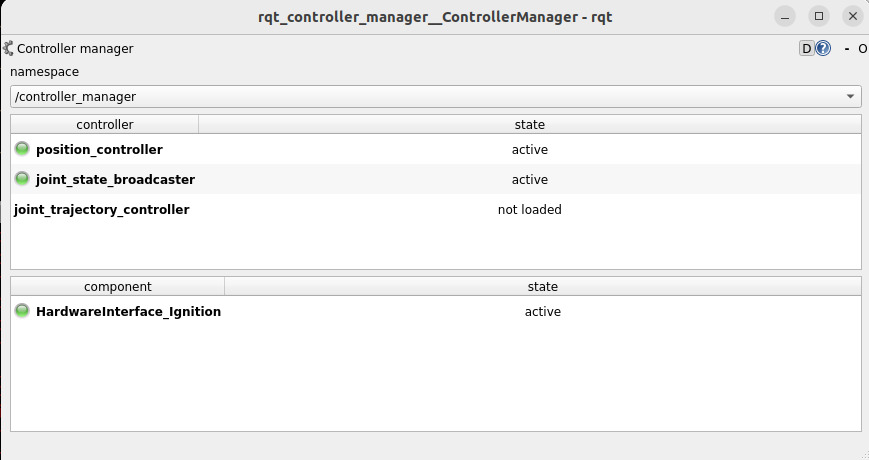
\includegraphics[width=1\textwidth]{Images/4D_7.jpeg} % nome file e larghezza

  \label{fig:publishCommand}
\end{figure}
\begin{figure}[H] % ✅ aggiunto [h!] per forzare il posizionamento
  \centering
  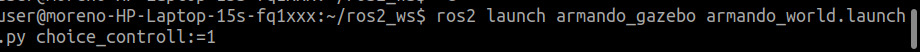
\includegraphics[width=1\textwidth]{Images/4D_8.jpeg} % nome file e larghezza

  \label{fig:publishCommand}
\end{figure}
\begin{figure}[H] % ✅ aggiunto [h!] per forzare il posizionamento
  \centering
  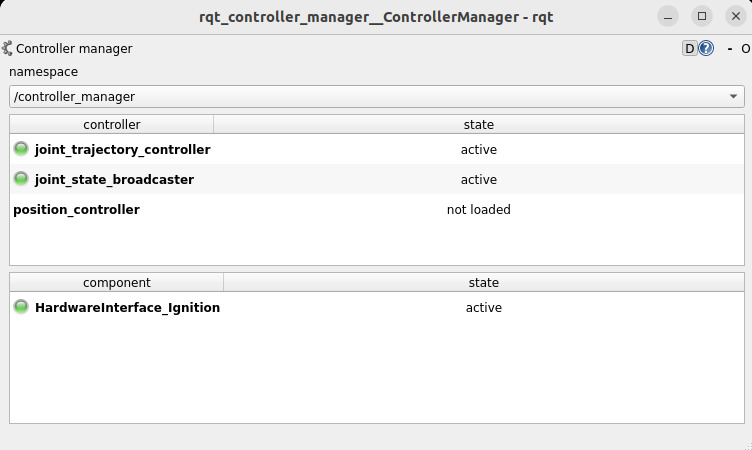
\includegraphics[width=1\textwidth]{Images/4D_9.jpeg} % nome file e larghezza

  \label{fig:publishCommand}
\end{figure}
\end{enumerate}

\end{document}
